\chapter{Abordagem Proposta} \label{chap:propApproach}
	\section{A Base de Sinais de Voz}
	    \subsection{Coleta dos Sinais}
		\par Para a realização desta pesquisa, coletou-se uma série de vozes nos arredores do Instituto de Biociências, Letras e Ciências Exatas da UNESP em São José do Rio Preto, no estado de São Paulo. Foram coletadas amostras de 21 indivíduos, das quais 20 foram usadas já que, em um dos casos, não foi possível coletar todos os dados necessários. Tais gravações se constituem de dígitos em um intervalo de 0 a 9 falados tanto em língua Inglesa quanto na Portuguesa. Os locutores foram escolhidos de acordo com seu sexo e idade de forma que a amostra estudada tenha uma abrangência que cubra desde crianças em época pré-escolar até adultos entre 50 e 60 anos dos sexos masculino e feminino.
					
		\par As gravações foram realizadas em ambientes distintos com diferentes níveis de ruído ao fundo, garantindo uma boa variabilidade de interferências corriqueiras, caracterizando casos reais. Foram usados arquivos no formato \textit{wav} sem compressão. A taxa de amostragem escolhida foi de 44100Hz, que permite, segundo o teorema de Nyquist, que seja realizada a quantização de frequências de até 22050Hz, com quantização de 16 bits.
		
		\par Coletados os sinais, os dígitos pronunciados nos mesmos foram separados um-a-um usando uma ferramenta desenvolvida para esse fim, resultando em um total de 410 sinais de voz de diferentes durações temporais que foram rotulados como ``genuínos''. Para cada um deles, foi criado um sinal ``espelho'',  regravado por um segundo dispositivo de gravação diferente do original, caracterizando os 410 sinais rotulados como ``regravados''.

	    \subsection{Organização da Base de Sinais}
		\par A organização da base de dados se deu por tipo, isto é, genuíno ou regravado, idioma, dígito ditado e interlocutor considerado. Foi criada uma estrutura hierárquica de diretórios de forma a permitir acesso fácil e intuitivo a cada um dos arquivos \textit{wav}, seja por vias automatizadas ou não. Os arquivos regravados residem no diretório ``playback'', enquanto que os genuínos se encontram no diretório ``live ''.	Essa organização está ilustrada nas Figuras \ref{fig:directorystructlevel01}, \ref{fig:directorystructlevel02} e \ref{fig:directorystructlevel03}.
		
		\par Para facilitar a automatização do processamento, foram criados três arquivos de texto:
		\begin{itemize}
			\item \textit{\textbf{dataSurvey.txt}}: contêm os dados de idade e sexo e nome do arquivo gerado para cada entrevistado;
			\item \textit{\textbf{inputListLive.txt}}: uma lista de caminhos para todos os arquivo não regravados;
			\item \textit{\textbf{inputListSpoofing.txt}}: apresenta uma listagem dos caminhos para todos os arquivos regravados.
		\end{itemize}
	
		\par Apenas para ilustrar, o conteúdo do diretório \textbf{``separated \textfractionsolidus live \textfractionsolidus en\_US \textfractionsolidus 0''} se constitui de vários arquivos do tipo \textit{wav}, cada um identificando o locutor ao qual pertence como exibido na Figura \ref{fig:directorystructlevel03}.

		\begin{figure}[ht]
			\centering
			\subfloat[0.3\textwidth][Base em nível 1]{
				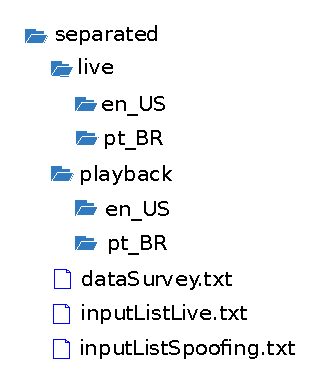
\includegraphics{images/directoryStructLevel01}
				\label{fig:directorystructlevel01}
			}
			\subfloat[0.3\textwidth][Base em nível 2]{
				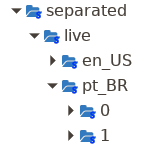
\includegraphics{images/directoryStructLevel02}
				\label{fig:directorystructlevel02}
			}
			\subfloat[0.3\textwidth][Base em nível 3]{
				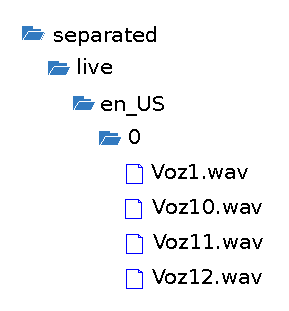
\includegraphics{images/directoryStructLevel03}
				\label{fig:directorystructlevel03}
			}
			\caption{Organização da base de dados}
			\label{fig:directorystructlevel010203}
		\end{figure}

	\section{Estrutura da Estratégia Proposta}
		\par A estratégia proposta para diferenciar sinais de voz genuínos daqueles regravados deu-se conforme ilustrado na Figura \ref{fig_arq}. Particularmente, a metodologia consiste na obtenção dos dados brutos de todos os 410 + 410 = 820 sinais de voz genuínos e regravados, seguida da conversão de cada um deles para um vetor de características correspondente, conforme explicado adiante. Na sequência, os melhores sub-conjuntos de características foram escolhidos com base na Engenharia Paraconsistente. Prosseguindo, separações aleatórias entre os vetores, com proporções diversas, foram realizadas para isolar aqueles destinados ao treinamento ou modelagem do classificador utilizado dos que foram destinados aos testes de classificação. Por fim, testes e resultados foram realizados, conforme descrito no Capítulo seguinte.
		
		\begin{figure}[h]
	\centering
	\caption{Estrutura da estratégia proposta}
	\scalebox{0.75}	{
		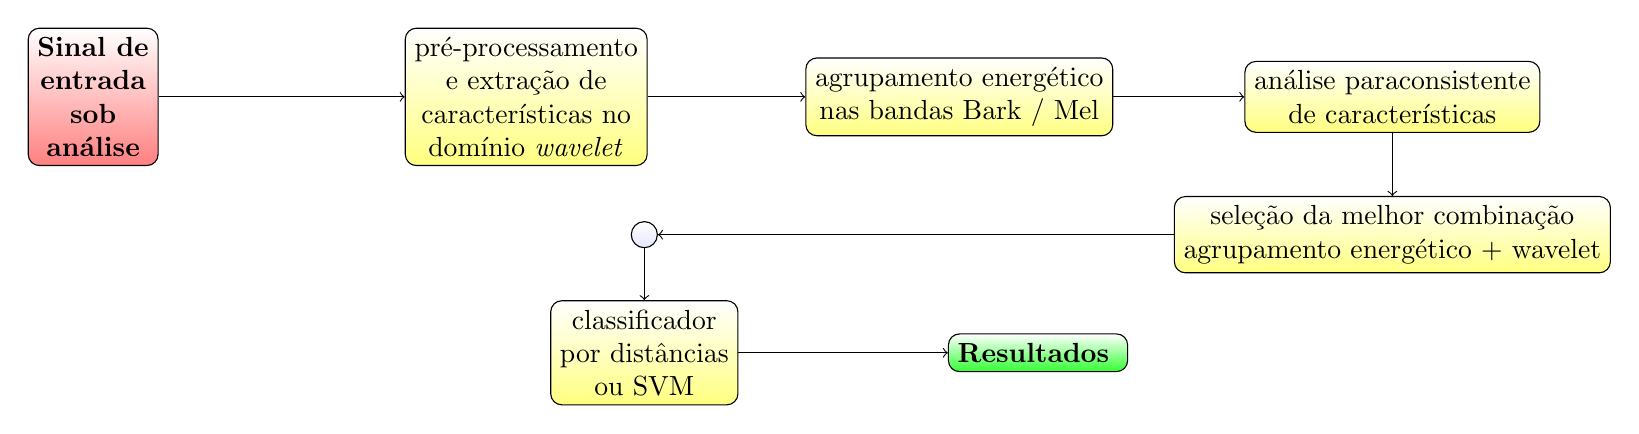
\begin{tikzpicture} 
			\node (z1)[shape=rectangle, rounded corners, draw, align=center, top color=white, bottom color=red!50] 
			at (0,2){
				\textbf{Sinal de} \\ \textbf{entrada} \\ \textbf{sob} \\ \textbf{análise}
			}; 
				
			\node (z2)[shape=rectangle, rounded corners, draw, align=center, top color=white, bottom color=yellow!50] 
			at (5.5,2){
				pré-processamento \\ e extração de \\ características no \\ domínio \textit{wavelet}
			}; 	
			
			\node (z3)[shape=rectangle, rounded corners, draw, align=center, top color=white, bottom color=yellow!50] 
			at (11,2){
				agrupamento energético \\ nas bandas Bark / Mel
			}; 	
			
			\node (z4)[shape=rectangle, rounded corners, draw, align=center, top color=white, bottom color=yellow!50] 
			at (16.5,2){
				análise paraconsistente \\ de características
			}; 
			
			\node (z5)[shape=rectangle, rounded corners, draw, align=center, top color=white, bottom color=yellow!50] 
			at (16.5,0.25){
				seleção da melhor combinação \\ agrupamento energético + wavelet
			}; 
					
			\node (z6)[shape=circle, draw, align=center, top color=white, bottom color=blue!10] 
			at (7,0.25) {};
			
			\node (z7)[shape=rectangle, rounded corners, draw, align=center, top color=white, bottom color=yellow!50] 
			at (7,-1.25) {
				classificador \\ por distâncias \\ ou SVM
			};
			
			\node (z8)[shape=rectangle, rounded corners, draw, align=center, top color=white, bottom color=green!80] 
			at (12,-1.25) {
				\textbf{Resultados}
			};
			
			\path[->] (z1) edge (z2);
			\path[->] (z2) edge (z3);
			\path[->] (z3) edge (z4);
			\path[->] (z4) edge (z5);
			\path[->] (z5) edge (z6);
			\path[->] (z6) edge (z7);	
			\path[->] (z7) edge (z8);
		\end{tikzpicture}
	}
	\label{fig_arq}
	\\Fonte: Elaborado pelo autor, 2021.
\end{figure}
		
		\par Conforme mencionado nos Capítulos anteriores, os vetores de características desta abordagem foram obtidos com base na Transformada \textit{Wavelet}, convertendo os sinais de voz do domínio do tempo para o domínio tempo-frequência. Particularmente, nos experimentos detalhados adiante, foram testados os seguintes filtros \textit{wavelet}: Haar, Daubechies de suportes 4 até 76, Symmlets com suportes 8, 16 e 32, Coiflets com suportes 6, 12, 18, 24 e 30, Beylkin com suporte 18 e, ainda, Vaidyanathan de suporte 24.

	\section{Procedimentos}
		\par Afim de garantir a comparação com outros trabalhos se fez necessário adotar várias formas de representar os resultados correspondentes para cada configuração experimental:
		\begin{itemize}
			\item Tabela de confusão.
			\item Acurácia e seu respectivo desvio padrão.
			\item EER (Equal Error Rate).
		\end{itemize}
		
		\par No exemplo constituído pela tabela de confusão \ref{tab:confusionMatrixSample} as \textbf{linhas} representam as \textbf{classes estimadas} e as \textbf{colunas} as \textbf{classes verdadeiras}, sendo que:
		\begin{itemize}
			\item \textbf{TP}: Quantidade de itens verdadeiros classificados como tal (\textit{True Positive}).
			\item \textbf{TN}: Quantidade de itens falsos classificados como tal (\textit{True Negative}).
			\item \textbf{FN}: Quantidade de itens verdadeiros classificados como falsos (\textit{False Negative}).
			\item \textbf{FP}: Quantidade de itens falsos classificados como verdadeiros (\textit{False Positive}).
		\end{itemize} 
		\begin{table}
\newcommand{\mc}[3]{\multicolumn{#1}{#2}{#3}}
\definecolor{tcB}{rgb}{0.447059,0.74902,0.266667}
\definecolor{tcC}{rgb}{0,0,0}
\definecolor{tcD}{rgb}{0,0.4,0.701961}
\definecolor{tcA}{rgb}{0.65098,0.65098,0.65098}
\begin{center}
	\begin{tabular}{ccc}
		% use packages: color,colortbl
		\mc{1}{l}{} & \mc{1}{>{\columncolor{tcA}}c}{\textbf{Verdadeiro}} & \mc{1}{>{\columncolor{tcA}}c}{\textbf{Falso}}\\

		\mc{1}{>{\columncolor{tcA}}r}{\textbf{Verdadeiro}} & \mc{1}{>{\columncolor{tcB}}c}{\textcolor{tcC}{VV}} & \mc{1}{>{\columncolor{tcD}}c}{\textcolor{tcC}{FV}}\\

		\mc{1}{>{\columncolor{tcA}}r}{\textbf{Falso}} & \mc{1}{>{\columncolor{tcD}}c}{\textcolor{tcC}{FF}} & \mc{1}{>{\columncolor{tcB}}c}{\textcolor{tcC}{VF}}
	\end{tabular}
	\caption{Exemplo de matriz de confusão}
	\label{tab:confusionMatrixSample}
\end{center}
\end{table}

		
		\par A acurácia usa os valores de \textit{TP}, \textit{TN} e a quantidade de elementos(\textit{N}) para ser calculada como mostrado na Equação \ref{eq:calculoDaAcuracia}.
		
		\begin{equation}
			acuracia = \dfrac{TP + TN}{N} \qquad.
			\label{eq:calculoDaAcuracia}
		\end{equation}

		\par Para se calcular o EER se leva em consideração os valores de \textit{FP} e \textit{FN} \cite{ghazali2018recent}, a partir desse valores são calculadas as \textit{False Acceptance Rate (\textbf{FAR})} representada na equação \ref{eq:FAR} e \textit{False Rejection Rate (\textbf{FRR})} representada por \ref{eq:FRR} ou \textbf{Taxa de falsos positivos} e \textbf{Taxa de falsos negativos} respectivamente.
		
		\begin{equation}
			FAR=\dfrac{FP}{TN+FP} \qquad.
			\label{eq:FAR}
		\end{equation}
		
		\begin{equation}
			FRR=\dfrac{FN}{FN+TP} \qquad.
			\label{eq:FRR}
		\end{equation}
				
		\par São calculadas tabelas de confusão por um número suficiente de vezes até que \textbf{\textit{FAR} seja igual \textit{FRR}}, a cada ciclo os vetores de características são comutados de forma aleatória para que se consiga valores diferentes, neste trabalho alguns casos precisaram de mais que 12000 iterações.
		
		\par Em cada iteração os valores de FAR e FRR são guardados em dois vetores, um para cada, então o vetor pertencente a FAR é ordenado de forma crescente e o outro decrescente. Esses pontos desenhados no gráfico juntamente com uma linha que divide o plano do mesmo ao meio tal que $x=y$ constituem o que se convencionou chamar de gráfico de \textit{Detection Error Tradeoff (DET)} ou, em tradução livre, \textbf{gráfico para balanceamento de erros}.
		
		\par O efetivo valor de \textbf{ERR se encontra na intersecção da reta $x=y$} com a curva definida por FAR e FRR como demonstrado no algoritmo \ref{lst:EERAlgo}.
	
		\begin{lstlisting}[language=C++, caption={EER algorithm}, label={lst:EERAlgo}]
double shortestDistance = highestValue();
double currentDistance = -highestValue();

double coordinateAboveDiagonalLine = { 0, 0 };
double coordinateBellowDiagonalLine = { 0, 0 };

sortAscending(FARVector);
sortDescending(FRRVector);

for (i = 0; i < FARVector.size(); i++) {
	// Calculate the distance between the coordinates defined
	// by the FAR and FRR vectors and the line defined by x=y
	currentDistance = absoluteValue((FARVector[i] - FRRVector[i]) / squaredRoot(2));
	
	// Stores just the shortest distance above the x=y line
	if (currentDistance <= shortestDistance && FRRVector[i] >= FARVector[i]) {
		shortestDistance = currentDistance;
		coordinateAboveDiagonalLine[0] = FARVector[i];
		coordinateAboveDiagonalLine[1] = FRRVector[i];
		jumpToNextIteration();
	}

	// Stores just the shortest distance bellow the x=y line
	coordinateBellowDiagonalLine[0] = FARVector[i];
	coordinateBellowDiagonalLine[1] = FRRVector[i];
	
	breakLoop();
}

// Calculates the intersection point of the curve defined by the FAR and FRR points and the x=y line
y = coordinateAboveDiagonalLine[0] - coordinateBellowDiagonalLine[0] - 1;
x = coordinateBellowDiagonalLine[1] - coordinateAboveDiagonalLine[1] + 1;
c = coordinateAboveDiagonalLine[1] * coordinateBellowDiagonalLine[0] - coordinateAboveDiagonalLine[0] * coordinateBellowDiagonalLine[1];

// Calculates the equal error rate
EER = -(c / (x + y));
\end{lstlisting}
	
		\subsection{Procedimento 01: filtros \textit{wavelet}, escalas Bark e Mel}
		\label{chap:propApproach:sec:Experimento01}
		\par O objetivo deste procedimento é o de verificar, segundo a Engenharia Paraconsistente, qual das combinações entre as escalas BARK ou MEL e as várias \textit{wavelets} consideradas geram os vetores de características mais propícios, ou seja, que atraem o ponto $(G_1,G_2)$ para uma posição mais próxima do vértice $(1,0)$ do plano paraconsistente, conforme mencionado no Capítulo anterior. 
				
		\par As transformações \textit{wavelet-packet} foram realizadas, com os diversos filtros mencionados, até  o máximo nível possível, implicando máxima resolução em frequência, para que, após isso, as amostras dos sinais transformados fossem agrupadas visando corresponder aos intervalos espectrais definidos nas escalas BARK e MEL. Naquela escala, os vetores de características foram constituídos de 24 coeficientes. Diferentemente, nesta escala, os vetores de características foram formados com 13 coeficientes devido a derivação do sinal ao final do processo de geração. O algoritmo \ref{lst:experiment01Algo} contém a descrição de tais procedimentos.
			
		\begin{lstlisting}[language=C++]
// Carregue para a memoria um dos conjuntos de amostra
for (listaDeAmostras : {listaComVoiceSpoofing, listaSemVoiceSpoofing}) {
	// Selecione o proximo tipo de wavelet
	for (wavelet : wavelets) {
		// Selecione entre BARK ou MEL
		for (barkOuMel : {BARK, MEL}) {
			// Selecione o proximo sinal dentro da amostra
			for (sinal : listaDeAmostras) {
				tamanhoOtimo=calcularTamanhoOtimo(sinal);
				redimensionar(sinal, tamanhoOtimo);
				sinalTransformado=wavelet(sinal, wavelet);
				energias=calcularEnergias(sinalTransformado, barkOuMel);
				energias=normalizar(energias);
				
				// Armazene os resultados
				resultados[wavelet.nome()][barkOuMel][listaDeAmostras.nome()].adicionar(energias);
			}
		}
	}
}
// Posicione os resultados no plano paraconsistente
mostraResultadosNoPlanoParaconsistente(resultados);
\end{lstlisting}

		\par Registre-se que, antes da aplicação da transformada \textit{wavelet-packet}, foi necessário redimensionar os sinais para que houvesse um comprimento correspondente a uma potência de 2, como indicado na equação \ref{eq:optimalSize}. Isso é necessário para que não haja perdas de trechos de voz ao final da transformação pois a transformada \textit{wavelet} realiza o \textit{downsampling} por 2, ou seja, em cada nível de decomposição o tamanho do vetor do sinal é diminuído pela metade. Caso haja um comprimento diferente do citado, em alguma parte do processo a divisão não será inteira fazendo com que algumas amostras dos sinais sejam perdidas.
				
		\par Para ajustar o tamanho do sinal de voz sob análise, foi usada a Equação \ref{eq:optimalSize}, na qual \textit{\textbf{proxInt}} é uma função que retorna o próximo número inteiro do argumento real. Por exemplo, $proxInt(1,5) = 2$.

		\begin{equation}
					tamanhoOtimo=2^{proxInt(\log_{2}tamanho)}
					\label{eq:optimalSize}
		\end{equation} 
		
		\par Após o redimensionamento do tamanho do sinal, o nível máximo de transformações é dado pela Equação \ref{eq:maxWaveletTransf}. 
				
		\begin{equation}
					maxTrans=\log_{2}(tamanho) \qquad.
					\label{eq:maxWaveletTransf}
		\end{equation}
		
		\subsection{Procedimento 02 - classificações baseadas em distâncias}
		\label{chap:propApproach:sec:Experimento02}
		\par O objetivo deste procedimento é verificar, considerando as melhores combinações descobertas pelo procedimento anterior, a acurácia de classificadores \textit{pattern-matching} por distâncias Euclidiana e Manhattan. Nesta fase, os vetores de características gerados pelo procedimento 01 são fornecidos aos classificadores para as mensurações devidas.
				
		\par Objetivando avaliar o comportamento dos classificadores com proporções múltiplas de 10\% da base de dados para modelagem, até o limite de 50\%, e o restante para testes, definiu-se que, para cada proporção, o sorteio aleatório para escolha dos vetores de características seria executado $n=t \cdot \frac{t+1}{2}$ vezes, sendo $t$ o número máximo de testes que podem ser realizados com uma certa porcentagem dos vetores. Em cada uma dessas execuções, a ordem dos vetores dentro das amostras, regravados e genuínos, foi permutada aleatoriamente.
				
		\par Para cada porcentagem foram coletadas as melhores e as piores acurácias assim como suas respectivas matrizes de confusão e assim calculadas suas \textit{EERs} conforme consta no Capítulo seguinte. No algoritmo \ref{lst:experiment02Algo}, os passos estão detalhados.
		
		\par Essencialmente, este procedimento 02 consiste em mensurar as distâncias entre cada vetor de características isolado para testes em relação à cada um dos vetores de características isolados para a modelagem, selecionando-se a menor delas. Em seguida, classifica-se o vetor de características que pertence aos testes e está sob análise, como pertencente à uma das classes dos vetores de modelagem selecionados.   
								
		\begin{lstlisting}[language=C++, caption={Procedure 02 algorithm}, label={lst:experiment02Algo}]
modelProportion={0.1, 0,2, 0,4, 0,5};
genuineModel = spoofingModel= genuineTest = spoofingTest = accuracyList = {};
for (distance : {Euclidian, Manhattan}) {
	for(percentage : modelProportion){
		for(testCounter = 0; testCounter < 300; testCounter++){
			// Choose feature vectors randomly from spoofing set
			// to build the model according to the proportions chosen.
			chooseRamdomly(voiceSpoofingSet, percentage, spoofingModel, spoofingTest);
			// Choose feature vectors randomly from genuine set
			// to build the tests according to the proportion chosen
			chooseRamdomly(genuineSet, percentage, genuineModel, genuineTest);
			
			trainClassificator("spoofing", spoofingModel);
			trainClassificator("genuine", genuineModel);
			// Classify the spoofing tests against the 
			// spoofing model and fill the confusion tables
			for(signal : spoofingTest){
				fillConfusionTable(signal, "spoofing");
			} 
			// Classify the genuine tests against the
			// genuine model and fill the confusion tables
			for(signal : genuineTest){
				fillConfusionTable(signal, "genuine");
			}

			accuracy=calculateAccuracy();
			
			// Store the accuracies for each percentage
			accuracyList[percentage].add(accuracy);

			// Store the best accuracy and its respective confusion table
			if(isTheBestAccuracy(accuracy)){
				saveAccuracyAndItsConfusionTable();
			}
			
			// Store the worst accuracy and its respective confusion table
			if(isTheWorstAccuracy(accuracy)){
				saveAccuracyAndItsConfusionTable();
			}
		}
		
		// Calculate and save the standard deviation for current proportion
		calculateAndSaveTheStandardDeviation(accuracyList[percentage]);
	}
}				
\end{lstlisting}

		\subsection{Procedimento 03 - classificações baseadas na SVM}
		\label{chap:propApproach:sec:Experimento03}
		\par Considerando as melhores combinações descobertas durante o procedimento 01, esta etapa visa medir a acurácia de uma SVM na separação das classes. O referido classificador foi escolhido pois estudos anteriores comprovam a sua eficácia para classificação binária \cite{bennett2000support}. 
		
		\par Particularmente, a estrutura da SVM utilizada foi definida da seguinte forma e de acordo com a Figura \ref{fig:3layersSVM}: 
		\begin{itemize}
		\item{}três camadas, sendo a primeira, isto é, de entrada, com elementos passivos, a segunda com elementos ativos não-lineares de núcleos Gaussianos e a terceira, isto é, a de saída, com um elemento ativo linear; 
		\item{}inexistem pesos entre a camada de entrada e a camada intermediária, implicando que a saída de cada elemento da camada de entrada conecta-se com todas as entradas de cada elemento da camada intermediária, mantendo incólumes os valores propagados;
		\item{}a saída de cada elemento da camada intermediária conecta-se com o único elemento da camada de saída por meio dos pesos $p_0, p_1, .... p_{X-1}$;
		\item{}o valor de saída consiste na combinação linear dos pesos com os valores recebidos como entrada da camada de saída, isto é, os valores de saída da camada intermediária.
		\end{itemize}
		
		\begin{figure}
	\centering
	\scalebox{2}{
				\begin{tikzpicture}
	%input layer
	\node (input1) at (0.65,2.0) {};
	\draw[->,in=180,out=0] (1.0,2.0) to (1.35,2.0);
	\node (input2) at (0.65,1.5) {};
	\draw[->,in=180,out=0] (1.0,1.5) to (1.35,1.5);
	\node (input3) at (0.65,1.0) {};
	\draw[->,in=180,out=0] (1.0,1.0) to (1.35,1.0);
	\node (input3) at (0.65,0.0) {};
	\draw[->,in=180,out=0] (1.0,0.0) to (1.35,0.0);
	\node (IL_N1) at (1.5,2.0) {}; \filldraw[fill=gray!30] (1.5,2.0) circle (0.15cm);
	\node (IL_N2) at (1.5,1.5) {}; \filldraw[fill=gray!30] (1.5,1.5) circle (0.15cm);
	\node (IL_N3) at (1.5,1.0) {}; \filldraw[fill=gray!30] (1.5,1.0) circle (0.15cm);
	\node at (1.5,0.625) {$\vdots$};
	\node (IL_Nn) at (1.5,0.0) {}; \filldraw[fill=gray!30] (1.5,0.0) circle (0.15cm);
	
	%hidden layer 
	\node (HL_N1) at (3.5,2.5) {}; \filldraw[fill=blue!20] (3.55,2.5) circle (0.15cm);
	\node (HL_N2) at (3.5,2.0) {}; \filldraw[fill=blue!20] (3.55,2.0) circle (0.15cm);
	\node (HL_N3) at (3.5,1.5) {}; \filldraw[fill=blue!20] (3.55,1.5) circle (0.15cm);
	\node (HL_N4) at (3.5,1.0) {}; \filldraw[fill=blue!20] (3.55,1.0) circle (0.15cm);
	\node at (3.55,0.625) {$\vdots$};
	\node (HL_Nn-1) at (3.5,0.0) {}; \filldraw[fill=blue!20] (3.55,0.0) circle (0.15cm);	
	\node (HL_Nn) at (3.5,-0.5) {}; \filldraw[fill=blue!20] (3.55,-0.5) circle (0.15cm);	
	\draw[->,in=180,out=0] (IL_N1)+(1.5mm,0) to (HL_N1);
	\draw[->,in=180,out=0] (IL_N1)+(1.5mm,0) to (HL_N2);
	\draw[->,in=180,out=0] (IL_N1)+(1.5mm,0) to (HL_N3);
	\draw[->,in=180,out=0] (IL_N1)+(1.5mm,0) to (HL_N4);
	\draw[->,in=180,out=0] (IL_N1)+(1.5mm,0) to (HL_Nn-1);
	\draw[->,in=180,out=0] (IL_N1)+(1.5mm,0) to (HL_Nn);
	
	\draw[->,in=180,out=0] (IL_N2)+(1.5mm,0) to (HL_N1);
	\draw[->,in=180,out=0] (IL_N2)+(1.5mm,0) to (HL_N2);
	\draw[->,in=180,out=0] (IL_N2)+(1.5mm,0) to (HL_N3);
	\draw[->,in=180,out=0] (IL_N2)+(1.5mm,0) to (HL_N4);
	\draw[->,in=180,out=0] (IL_N2)+(1.5mm,0) to (HL_Nn-1);
	\draw[->,in=180,out=0] (IL_N2)+(1.5mm,0) to (HL_Nn);
	
	\draw[->,in=180,out=0] (IL_N3)+(1.5mm,0) to (HL_N1);
	\draw[->,in=180,out=0] (IL_N3)+(1.5mm,0) to (HL_N2);
	\draw[->,in=180,out=0] (IL_N3)+(1.5mm,0) to (HL_N3);
	\draw[->,in=180,out=0] (IL_N3)+(1.5mm,0) to (HL_N4);
	\draw[->,in=180,out=0] (IL_N3)+(1.5mm,0) to (HL_Nn-1);
	\draw[->,in=180,out=0] (IL_N3)+(1.5mm,0) to (HL_Nn);
	
	\draw[->,in=180,out=0] (IL_Nn)+(1.5mm,0) to (HL_N1);
	\draw[->,in=180,out=0] (IL_Nn)+(1.5mm,0) to (HL_N2);
	\draw[->,in=180,out=0] (IL_Nn)+(1.5mm,0) to (HL_N3);
	\draw[->,in=180,out=0] (IL_Nn)+(1.5mm,0) to (HL_N4);
	\draw[->,in=180,out=0] (IL_Nn)+(1.5mm,0) to (HL_Nn-1);
	\draw[->,in=180,out=0] (IL_Nn)+(1.5mm,0) to (HL_Nn);
	
	%output layer
	\node (OL_N1) at (5.5,1.0) {}; \filldraw[fill=red!40] (5.55,1.0) circle (0.15cm);
	
	\draw[->,in=180,out=0] (HL_N1)+(2mm,0) to (OL_N1);
	\draw[->,in=180,out=0] (HL_N2)+(2mm,0) to (OL_N1);
	\draw[->,in=180,out=0] (HL_N3)+(2mm,0) to (OL_N1);
	\draw[->,in=180,out=0] (HL_N4)+(2mm,0) to (OL_N1);
	\draw[->,in=180,out=0] (HL_Nn-1)+(2mm,0) to (OL_N1);
	\draw[->,in=180,out=0] (HL_Nn)+(2mm,0) to (OL_N1);
	%
	\draw[snake=brace,mirror snake,raise snake=45pt,brown] (1.25,1.25) -- (1.75,1.25) node[black,midway,yshift=-50pt,below]{\tiny camada de} node[black,midway,yshift=-58pt,below]{\tiny entrada com} node[black,midway,yshift=-66pt,below]{\tiny $R$ elementos}
	node[black,midway,yshift=-74pt,below]{\tiny passivos};
	\draw[snake=brace,mirror snake,raise snake=45pt,brown] (3.25,0.75) -- (3.75,0.75) node[black,midway,yshift=-50pt,below]{\tiny camada} node[black,midway,yshift=-58pt,below]{\tiny intermediária} node[black,midway,yshift=-66pt,below]{\tiny com $X$ neurônios}
	node[black,midway,yshift=-74pt,below]{\tiny ativos não-lineares};
	\draw[snake=brace,mirror snake,raise snake=45pt,brown] (5.25,1.75) -- (5.75,1.75) node[black,midway,yshift=-50pt,below]{\tiny camada de} node[black,midway,yshift=-58pt,below]{\tiny saída com} node[black,midway,yshift=-66pt,below]{\tiny um elemento}
	node[black,midway,yshift=-74pt,below]{\tiny ativo linear};
	%
	\node (OUT) at (6.5,1.0) {\tiny resultado}; 
	\draw[->,in=180,out=0] (OL_N1)+(2mm,0) to (OUT);	
	
	\node at (4,2.6) {\tiny $p_0$}; 
	\node at (4,2.1) {\tiny $p_1$}; 
	\node at (4,1.65) {\tiny $p_2$}; 
	\node at (4,1.2) {\tiny $p_3$}; 
	\node at (4,0.2) {\tiny $p_{X-2}$}; 
	\node at (4,-0.3) {\tiny $p_{X-1}$}; 
\end{tikzpicture}
	}
	\caption{Estrutura da SVM para o procedimento 03 com $R$ neurônios na camada de entrada, sendo $R$ a dimensão dos vetores de características, e $X$ neurônios na camada intermediária, sendo $X$ o número de casos de treinamento}
	\label{fig:3layersSVM}
\end{figure} 

		\par Foram utilizados, na camada de entrada, um número de elementos igual a dimensão do vetor de características sendo considerado. Na camada intermediária, o número de elementos ativos não-lineares foi igual ao número de casos de treinamento, visando facilitar o procedimento que, em tal caso, implica na solução direta de um sistema linear quadrado, isto é, possível e determinado \cite{poole2014linear}. 
		
		\par O treinamento da SVM consiste em, numa primeira etapa não-supervisionada, ajustar os parâmetros das funções Gaussianas da camada intermediária. Posteriormente, com base no sistema linear mencionado, os pesos foram encontrados com base em uma abordagem supervisionada, utilizando-se os rótulos -1 e 1 para os sinais regravados e genuínos, respectivamente.    
		
		\par Todos os arranjos para a seleção dos vetores de treinamento e testes, assim como demais detalhes,   são idênticos àqueles do procedimento 02 e encontram-se listados no algoritmo \ref{lst:experiment03Algo}. 
		
		\begin{lstlisting}[language=C++, caption={Algoritmo que caracteriza o procedimento 03}, label={lst:experiment03Algo}]
tamanhosDoModelo={0.1, 0,2, 0,4, 0,5};
modeloDeReferenciaNaoSpoofing={};
modeloDeReferenciaSpoofing={};
testesNaoSpoofing={};
testesSpoofing={};
	for(porcentagem : tamanhosDoModelo){
		for(teste = 0; teste < 300; teste++){
			// Escolhe aleatoriamente os sinais para o modelo com spoofing 
			// e os grava em 'modeloDeReferenciaSpoofing' o restante vai 
			// para 'testesSpoofing'
			escolherAleatoriamente(listaComVoiceSpoofing, porcentagem, modeloDeReferenciaSpoofing, testesSpoofing);
			
			// Escolhe aleatoriamente os sinais para o modelo sem spoofing
			// e os grava em 'modeloDeReferenciaNaoSpoofing' o restante vai 
			// para 'testesNaoSpoofing'
			escolherAleatoriamente(listaSemVoiceSpoofing, porcentagem, modeloDeReferenciaNaoSpoofing, testesNaoSpoofing);
			treinarClassificador("spoofing", modeloDeReferenciaSpoofing);
			treinarClassificador("naoSpoofing", modeloDeReferenciaNaoSpoofing);
			
			// Classifica os testes e preenche a tabela de confusao
			for(sinal : testesSpoofing){
				preencherTabelaDeConfusao(sinal, "spoofing");
			} 
			
			// Classifica os testes e preenche a tabela de confusao
			for(sinal : testesNaoSpoofing){
				preencherTabelaDeConfusao(sinal, "naoSpoofing");
			}
			
			acuracia=calculaAcuracia();
			
			// Salva a melhor acuracia e matriz de confusao
			if(ehAMelhorAcuracia(acuracia)){
				salvaAcuraciaEMatrizDeConfusao();
			}
			
			// Salva a pior acuracia e matriz de confusao
			if(ehAPiorAcuracia(acuracia)){
				salvaAcuraciaEMatrizDeConfusao();
			}
		}
	}			
\end{lstlisting}

        \par Os testes e resultados dos experimentos descritos neste Capítulo encontram-se no Capítulo seguinte. 